
\chapter{Using the software\label{chapter:using}}
\noindent The GNN classifier was implemented in GNU Octave 3.6.2 and tested on a x86\_64 PC. The most important functions are:
\begin{itemize}
	\item loadgraph - loads a single graph from .csv files
	\item loadset - loads a set of graphs sharing the same filename prefix
	\item mergegraphs - merge a cellarray of graphs to a single graph
	\item initgnn - initialize a new GNN
	\item traingnn - train GNN using a training graph
	\item classifygnn - classify given graph with a trained GNN
	\item evaluate - evaluate the classification results
	\item crossvalidate - perform cross-validation using an untrained GNN and a set of graphs
\end{itemize}
\noindent Help and usage information for each function can be displayed by typing \emph{help <function\_name>} in the Octave command line.\\



\begin{lstlisting}[style=outcode, language=Matlab, caption=Sample usage session]
g6 = loadset('../data/g6s3n/g6s3', 10);
gm = mergegraphs(g6);
gnn = initgnn(gm.maxIndegree, [5 5], [5 gm.nodeOutputSize], 'tansig');
trainedGnn = traingnn(gnn, gm, 20);
outputs = classifygnn(trainedGnn, gm);
stats = evaluate(outputs, gm.expectedOutput);
\end{lstlisting}

\noindent All subgraph matching datasets were created using the \emph{buildgraphs.py} script. Each graph can be viewed as a pdf file by using the \emph{drawgraph.py} script. Each graph is stored as three .csv files, containing node labels, edge labels and expected outputs. A sample graph \emph{'test'} is presented below. Nodes yielding output 2 were marked as black.

\begin{figure}
\begin{floatrow}
\ffigbox[\FBwidth]{	% use the image width
	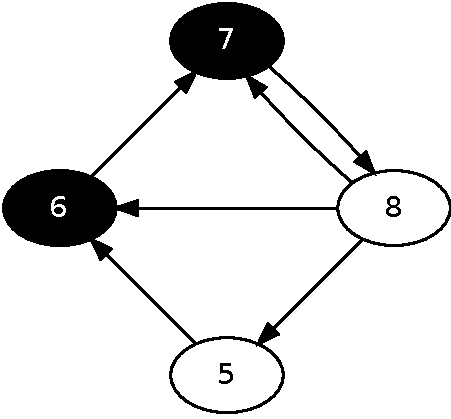
\includegraphics[scale=0.55]{img/test}
}{
\caption{Sample graph}
}
\capbtabbox{
	\begin{tabular}{lll}
	\toprule
	test\_nodes.csv & test\_output.csv & test\_edges.csv \\
	\midrule
	5	&	1	&	1,2,0\\
	6	&	2	&	2,3,0\\
	7	&	2	&	3,4,0\\
	8	&	1	&	4,1,0\\
		&		&	4,2,0\\
		&		&	4,3,0\\
	\bottomrule
	\end{tabular}
}{
\caption{Sample graph data}%
}
\end{floatrow}
\end{figure}
